\chapter{Data}\label{chap:data}

\section{Interlinear Examples}\label{sec:interlinear}
Format interlinear examples using the shorthand codes \verb|\ea|  and \verb|\z|. Each instance of  \verb|\ea| must be closed with \verb|\z|. The following codes results in the example formatted as \REF{ex:balantak}. If you need to align multiple words with a single gloss, put the words in curly braces \verb|{ }|. 

{\small 
\begin{lstlisting} 
\ea  Example heading \label{ex:example label} \\
\gll example text \\
interlinear gloss \\
\glt `free translation' 
\z
\end{lstlisting}
}

\noindent
Note the double backslashes \verb|\\| (line break) following the label and following both the example and gloss  lines. There is \textit{no} double backslash following the free translation line.

\ea  Balantak elevational deixis \citep[134]{busenitz1992}\label{ex:balantak}\\
\gll I-ro'o na intu-na woo' i-ya'a \\
{extension-\low} prep under-\gloss{3SG:POSS} areca extension-\gloss{DEM} \\
\glt `that person down there underneath that areca palm' 
\z

\noindent
Format an example with subexamples as follows by embedding another ea command followed by ex for subsequent subparts. 

{\small \begin{lstlisting}

\ea Example title \label{ex:label}  % note no \\ here
\ea \gll example text \\
interlinear gloss \\
\glt `free translation' 
\ex \gll example text \\.  % note  \ex not \ea here
interlinear gloss \\
\glt `free translation' 
\z\z
\end{lstlisting} }


\noindent
You can reference just one part of the example by supplying the letter(s) referring to the example part in square brackets with the \verb|\REF[]{}| command. Note this only works with uppercase \verb|\REF|, not lowercase \verb|\ref|. Thus, 
\verb|\REF[b]{ex:busang}|
produces a reference to \REF[b]{ex:busang} below.

\ea Busang cardinal direction terms \citep[29]{barth1910}\label{ex:busang}  % note no double backslash here
\ea \gll Bèh ulé mata n dó muun\\
side left eye \gl{gen} sun rise\\
\glt `north' (literally, `left of the rising sun')   
\ex \gll Bèh ulé mata n dó uli\\
side left eye \gl{gen} sun return\\
\glt `south' (literally, `left of the setting sun') 
\z\z


\section{Tables}\label{sec:tables}
Use the \verb|table| environment to create simple tables. Specify the columns and alignment as arguments of the \verb|tabular| environment. Table~\ref{tab:ambel} has 6 columns. The first is left-aligned, the others are center-aligned. 
Note that  you can use the [h] option to ask {\LaTeX} to try to place your tables (and figures) inline, but the resulting table may not always be inline. This can be one of the most frustrating features of {\LaTeX} for users coming from a word processing background. There are various workarounds. 

\begin{table}[h]
    \centering\small
    \begin{tabular}{l|ccccc}
        \toprule
            & prefix & \gl{prox} & \gl{mid} & \gl{dist} & \gl{and}\\
            \midrule
            ‘seaward' & lu- & lune & lupa & luma & lua \\
            ‘landward’ & li- & line &  lipa &  lima & lia\\
            ‘up, out’ & i- & ine & ipa & ima & ia\\
            ‘down’ & pu- & pune &  pupa & puma & pua\\
            ‘front’& ta(y)- & tane & tapa & tama & taya \\
            ‘in, back’ & mu- &  mune & mupa & muma & mua\\
            `side' & pa(y)- & pane & papa & pama & paya \\
        \bottomrule
    \end{tabular}   
    \caption{Directional terms in Ambel (Waigeo) 
    \citep[489]{arnold2018}.}
    \label{tab:ambel}
\end{table}

\noindent
\verb|\multirow| and \verb|\multicolumn| can be used to span rows and columns, respectively, as in Table~\ref{tab:sangir}.


\begin{table}[h]
    \centering\small
    \begin{tabular}{l|ccc}
        \toprule
         & \gl{loc}&\gl{trans}&\gl{cis}  \\ \midrule
        similar level & pai & tamai &damahi \\ \hline
        back-, inland-,  somewhat upward & dala & \multirow{2}{*}{taraiʔ} & \multirow{2}{*}{ɨndaiʔ}  \\
        upward & dasiʔ &&\\ \hline
        front-, coast-,  somewhat downward & dadeʔ & \multirow{2}{*}{tanaeʔ} & \multirow{2}{*}{ɨnnaeʔ}\\ 
        downward &  baβa &&\\ \hline
        seaward & -- & sasaeʔ & ɨnsaeʔ\\
        \bottomrule
    \end{tabular}
    \caption{ Sangir elevational terms, showing forms for a stationary entity (\gl{locative}), movement away from speaker (\gl{translocative}), and movement toward speaker (\gl{cislocative}) (after \citealt{jukes2015}).  }
    \label{tab:sangir}
\end{table}

\section{Figures}\label{sec:figures}

Place image files in the figures folder. Then insert them into the document using the \verb|figure| environment. Specify the width of the figure using the width option. This can be a measurement such as 4cm or 5in, but it is often convenient to use a fraction of the \verb|\textwidth| on the page, as in Figure~\ref{fig:embaloh}.

{\small 
\begin{lstlisting}
\begin{figure}[h]
    \centering
    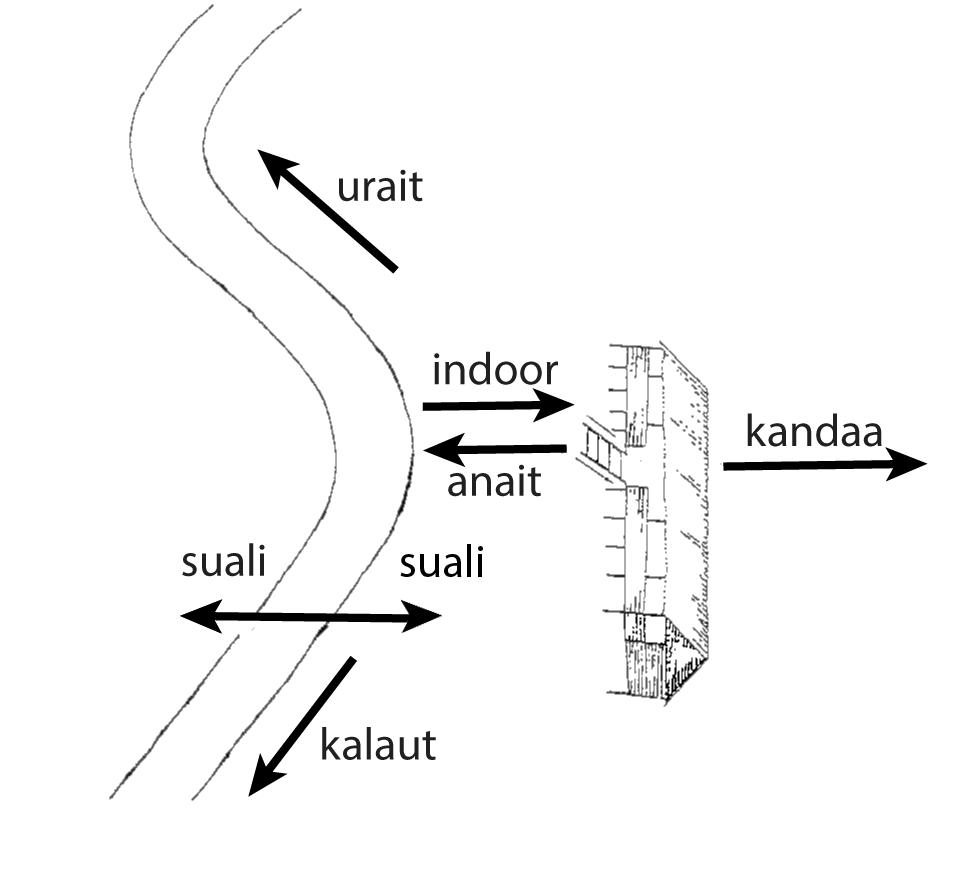
\includegraphics[width=mywidth]{myfig}
    \caption{My Caption}
    \label{fig:my_label}
\end{figure}
\end{lstlisting}}



\begin{figure}[h]
    \centering
    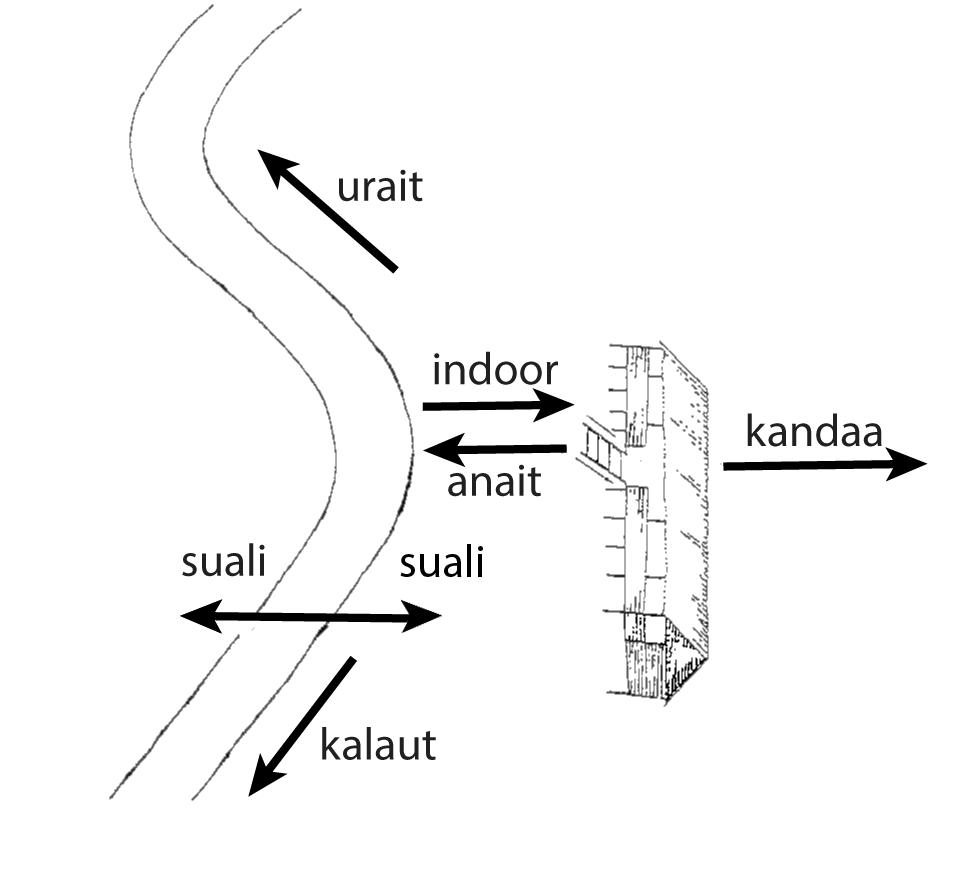
\includegraphics[width=0.5\textwidth]{myfig}
    \caption{Embaloh riverine directional terms \citep[after][70]{adelaar1997}.}
    \label{fig:embaloh}
\end{figure}


